%% FeatureLiftBench: FSE-oriented condensed manuscript, revised 2026-09-16.
%% Scope: Python-150 benchmark; 150 tasks x 6 configurations (900 outcomes).
%% Current inputs and model configurations: paper_sources.json.
\documentclass[acmsmall,screen,review,anonymous]{acmart}

\usepackage{amsmath}
\usepackage{booktabs}
\usepackage{tabularx}
\usepackage{graphicx}
\usepackage{xspace}
\usepackage{microtype}
\usepackage{placeins}

\newcommand{\flb}{\textsc{FeatureLiftBench}\xspace}
\newcommand{\rres}{\textsc{RRES}\xspace}
\graphicspath{{figures/}}
\setlength{\emergencystretch}{2em}
\citestyle{acmauthoryear}

\begin{document}

\title[FeatureLiftBench: Behavior-Preserving Feature Lifting]{FeatureLiftBench: Benchmarking Behavior-Preserving Feature Lifting from Real Repositories}
\author{Anonymous Author(s)}

\begin{abstract}
Reusing existing software often requires moving a capability beyond its original
project boundary while preserving its behavior. We introduce \flb, a benchmark
for \emph{behavior-preserving feature lifting}: given an intact, version-pinned
source repository and a public behavioral contract, a coding agent constructs an
independent package that is evaluated without runtime access to the source
repository. \flb contains 150 Python tasks from 126 repositories and 132 source
snapshots. Benchmark validation combines automated consistency checks, semantic
review of all 150 retained tasks by multiple authors supported by AI-assisted
evidence, and 450 passing source-free reference replays. We evaluate six model--harness
configurations on the same task set; functional pass rates range from 24.0\% to
76.7\%. The two strongest configurations deliver packages for every task, yet 76
of their 77 combined failures first emerge at behavioral gates. A paired 40-task
ablation shows that repository evidence raises GPT-5.6 Luna's success from 22.5\%
to 57.5\% and Qwen's from 2.5\% to 30.0\%; every Full-only success for these two
configurations corresponds to a behaviorally failing Contract-Only artifact.
However, 241 of 303 behavioral-first failures in the main comparison already
contain confirmed reads of entrypoint-associated source files. Repository
evidence therefore materially helps reconstruction, but availability and
observed source exposure are not sufficient for behavior preservation. Successful
artifacts also vary substantially in implementation size and retained source
overlap. \flb isolates behavior preservation across a new software boundary as a
distinct challenge for repository-level coding agents.
\end{abstract}

\begin{CCSXML}
<ccs2012>
 <concept><concept_id>10011007.10011074.10011099.10011102</concept_id>
 <concept_desc>Software and its engineering~Software testing and debugging</concept_desc>
 <concept_significance>500</concept_significance></concept>
 <concept><concept_id>10011007.10011074.10011099</concept_id>
 <concept_desc>Software and its engineering~Software verification and validation</concept_desc>
 <concept_significance>300</concept_significance></concept>
</ccs2012>
\end{CCSXML}
\ccsdesc[500]{Software and its engineering~Software testing and debugging}
\ccsdesc[300]{Software and its engineering~Software verification and validation}
\keywords{coding agents, software reuse, feature extraction, behavioral preservation, benchmark}
\maketitle

\section{Introduction}
\label{sec:introduction}

Software reuse involves selecting, adapting, and integrating existing
artifacts~\cite{krueger1992reuse}. Moving a capability across project boundaries
is one such reuse scenario: a developer may need a parser from a larger tool, configuration
handling from a framework, or a signal registry for a new library. Although the
source implementation is available, the target capability may extend beyond any
single file or function: its behavior can depend on supporting modules, shared
state, framework mechanisms, configuration, and packaged resources. Reuse
therefore requires more than locating code. The relevant behavior must be
reconstructed so that it continues to hold after the original project context is
removed. This raises a practical question: \emph{can a coding agent use an intact
source repository to deliver a specified capability as a behaviorally correct,
independently executable package?}

We formulate this task as \emph{behavior-preserving feature lifting}, or
\emph{feature lifting} for short. Given a version-pinned source repository and a
public behavioral contract, an agent constructs a new package that is evaluated
without runtime access to the source repository. The agent may extract, adapt, or
reimplement code; correctness is determined by the observable behavior required
at the new package boundary. Feature lifting therefore couples repository
understanding with software reuse: the implementation is available as evidence,
but the resulting capability must survive outside the environment that originally
supported it. Figure~\ref{fig:pipeline} illustrates this setting.

\begin{figure}[tbp]
  \centering
  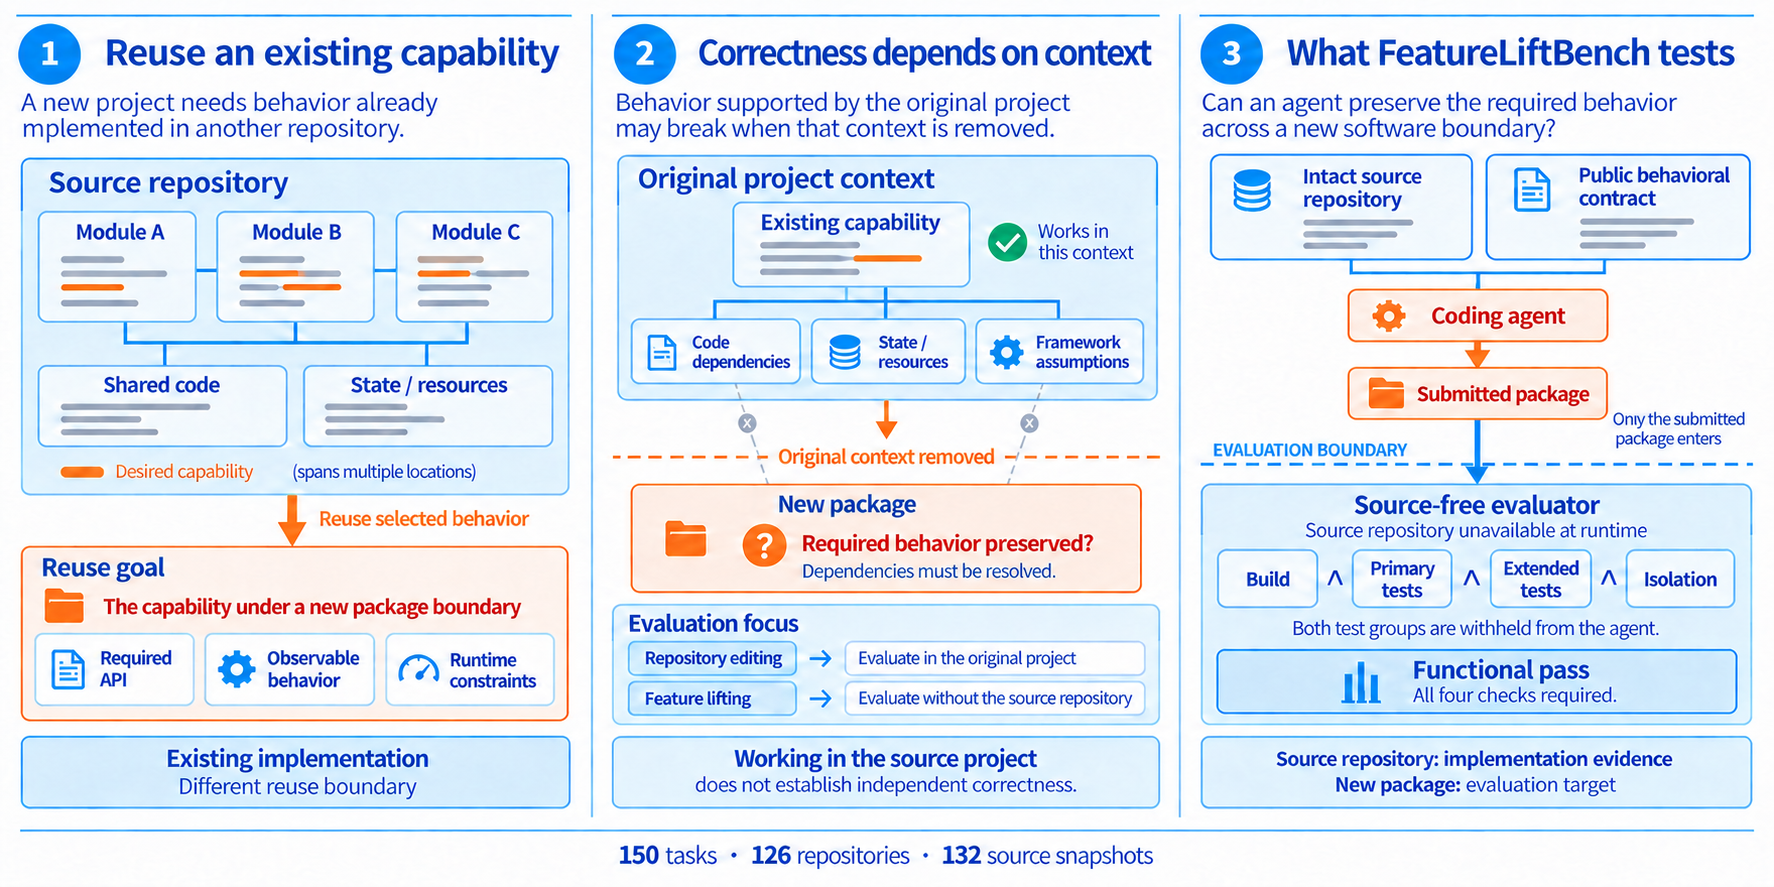
\includegraphics[width=\linewidth]{figures/fig1.png}
  \caption{Motivation and task overview of \flb. An agent receives the intact
  source repository and a public behavioral contract, constructs a new package,
  and submits only that package to source-free evaluation. The repository
  structure and highlighted locations are illustrative; agents receive no
  benchmark-provided source-location hints.}
  \Description{Three panels show a source capability supported by multiple
  repository components, reconstruction into a new package, and source-free
  evaluation of the submitted package.}
  \label{fig:pipeline}
\end{figure}

This setting differs from two common forms of repository-level evaluation.
SWE-bench and SWE-Bench Pro ask agents to modify an existing project in response
to an issue~\cite{jimenez2024swebench,deng2025swebenchpro}, while FeatBench and
FeatureBench study feature implementation in an existing or partially removed
codebase~\cite{chen2026featbench,zhou2026featurebench}. In feature lifting, by
contrast, the complete implementation of the target capability is intentionally
available as evidence, but the deliverable is a new independent package whose
behavior is evaluated without the donor repository. This also differs from
classical software transplantation, which extracts donor functionality for
integration into a supplied host program~\cite{barr2015transplantation}. Our
focus is the general coding-agent setting in which the destination boundary is a
standalone package and the extraction strategy is left open.

To study this problem, we introduce \flb, a benchmark of 150 Python tasks drawn
from 126 repositories and 132 pinned source snapshots. Each task provides the
complete source repository and a public behavioral contract, while withholding
benchmark tests, reference implementations, and source-location hints. Submitted
packages are evaluated through loading, behavioral, and source-isolation checks
without the source repository. Benchmark construction combines explicit
contracts and protected tests with automated consistency checks, semantic review
of all 150 retained tasks by multiple authors supported by AI-assisted evidence,
and repeated execution of feasible reference implementations.

We evaluate six model--harness configurations on the same 150 tasks and observe
substantial but incomplete capability: functional pass rates range from 24.0\%
to 76.7\%. For the two strongest configurations, DeepSeek V4 Pro and Flash, all
150 tasks receive usable submissions, yet 76 of their 77 combined failures first
occur at behavioral gates rather than during delivery or loading. A paired
source-evidence ablation further shows that intact repository evidence materially
improves reconstruction: GPT-5.6 Luna gains 35.0 percentage points and Qwen gains
27.5 points over Contract Only. However, source access is not sufficient by
itself. Among 303 behavioral-first failures in the main comparison, 241 (79.5\%)
already contain confirmed reads returning content from entrypoint-associated
source files. Successful artifacts also differ substantially in implementation
footprint, motivating us to characterize size and retained source overlap only
after functional correctness has been established. Retrospective trajectory
analysis additionally examines execution that continues after an observed passing
artifact, beyond what final success rates alone describe.

This work makes three contributions:
\begin{itemize}
  \item \textbf{A task formulation for behavior-preserving feature lifting.}
  We define a repository-level reuse setting in which intact implementation
  evidence is available during construction, but the requested capability must
  execute across a new, source-free package boundary.

  \item \textbf{FeatureLiftBench, an executable benchmark of real repository
  reuse.} We construct and validate 150 tasks from 126 Python repositories,
  combining bounded behavioral contracts, protected tests, source-free
  evaluation, multi-author semantic review, and repeated reference execution.

  \item \textbf{An empirical study of current coding agents.}
  We compare six configurations on the full benchmark, measure the effect of
  repository evidence through paired ablation, diagnose behavioral failures
  after observed source exposure, and characterize the implementation footprint
  of functionally successful artifacts, together with execution effort before
  and after an observed passing checkpoint.
\end{itemize}

\section{The FeatureLiftBench Benchmark}
\label{sec:benchmark}

\flb comprises 150 executable feature-lifting tasks. Each task connects an
existing capability in a complete source repository to a public contract for a
new package. The agent receives implementation evidence and the contract; the
submitted package is assessed by protected behavioral tests in a source-free
environment. A reference implementation provides evidence that the task is
feasible. We first define the task and its visibility boundary, then describe
construction, validation, and benchmark composition.

\subsection{Task Formulation and Running Example}

A \flb task consists of a pinned source repository $R$, a public behavioral
contract $S$, an initial workspace $W$, and a protected evaluator $J$. A model
backend $M$ acting through an agent harness $H$ produces a submitted artifact
$A$:
\begin{equation}
  A = \operatorname{Run}(M,H,R,S,W).
\end{equation}

We use a behavioral contract to make interface obligations
explicit~\cite{meyer1992contract}. It specifies the required API surface and observable behavior,
including relevant defaults, exceptions, state changes, ordering constraints,
and explicit exclusions. The agent may inspect the complete pinned repository,
including upstream tests and documentation, but must construct the result in a
designated submission directory. Benchmark tests, reference implementations,
test-to-contract mappings, and benchmark-provided source-location hints remain
hidden.

The required output is an independently executable package under the benchmark
environment. The package may extract, adapt, or reimplement upstream code, but
it must execute without runtime access to the source repository. The contract,
rather than any particular source slice, defines the preservation boundary.
Consequently, multiple structurally different implementations may satisfy the
same task.

Functional success is defined as
\begin{equation}
  F(A)=B(A)\land T_{\mathrm{primary}}(A)
       \land T_{\mathrm{extended}}(A)\land I(A),
  \label{eq:functional}
\end{equation}
where $B$ checks that the submitted package can be loaded under the frozen
evaluation environment, $T_{\mathrm{primary}}$ and
$T_{\mathrm{extended}}$ exercise protected behavioral obligations, and $I$
checks source independence. All four conditions must hold.

\paragraph{Running example: a signal registry.}
The Blinker task asks the agent to reconstruct \texttt{Signal} and
\texttt{Namespace} under a new package boundary. Its contract requires behavior
such as sender-specific dispatch, weak-receiver cleanup, stable namespace
identity, and scoped connection management, while explicitly excluding
asynchronous dispatch and the upstream global named-signal singleton. Thus, an
implementation whose central \texttt{connect} and \texttt{send} paths work can
still fail if supporting state or lifetime behavior is lost. The agent may reuse
or reimplement the relevant upstream logic, but the resulting package must
satisfy the contract without importing or reading the original \texttt{blinker}
source at runtime.

\subsection{Task Construction}
\label{sec:construction}

Construction turns an existing repository capability into a bounded,
source-backed lifting task with a public behavioral contract, protected tests,
and a feasible source-independent reference implementation.
Figure~\ref{fig:construction} summarizes the construction and validation
workflow.

\paragraph{Select a capability and pin its source.}
We select capabilities from Python libraries, developer tools, and framework
components when their observable behavior can be stated explicitly and executed
without live external services. Each task is tied to a pinned source snapshot.
Agents receive the complete tracked source tree, including upstream tests and
documentation, rather than a feature-specific slice. Identifying the relevant
implementation and its supporting dependencies therefore remains part of the
task.

\paragraph{Define the behavioral contract.}
For each capability, we specify the exported APIs and the observable behavior
that must be preserved, including relevant signatures, defaults, exceptions,
state changes, and explicit exclusions. The contract may also declare an
adaptation when the requested package interface intentionally differs from the
upstream capability. The resulting task statement describes what the package
must do without prescribing where the implementation resides or how it should
be reconstructed; benchmark-provided source-location hints are withheld.

\paragraph{Construct protected tests and a feasible reference.}
Primary and Extended test groups operationalize the same public contract:
Primary covers central obligations, while Extended exercises additional cases
and combinations without introducing new requirements. Both groups are hidden
from the agent. Test-to-contract mappings are maintained during construction to
check that evaluator expectations remain within the declared boundary.

For each task, we also retain a reference package that passes the same
source-free functional evaluation as agent submissions. References may be
constructed by extracting and adapting upstream code or by task-specific
implementation. They establish that the task is executable under the benchmark
environment and provide a reference point for artifact-size measurements; they
are neither unique solutions nor proofs of a minimum behavioral closure.

\paragraph{Freeze the benchmark.}
After validation, task specifications, pinned source identities, protected
tests, reference packages, dependency policies, and evaluator settings are
versioned together. The frozen benchmark contains 150 tasks from 126
repositories and 132 source snapshots. The same 150-task membership is used for
every configuration in the main comparison.

\subsection{Benchmark Validation}
\label{sec:validation}

Validation must address whether evaluator judgments capture the intended
behavior, an instance of the test-oracle problem~\cite{barr2015oracle}.
We validate the frozen benchmark at three complementary levels: structural
consistency, semantic alignment, and executable feasibility.

\paragraph{Structural consistency.}
Automated checks verify required task assets, source mappings, dependency
declarations, generated task statements, and test-to-contract mappings. All 150
retained task packages pass these checks and resolve to 132 verified source
snapshots. These checks target inconsistencies such as stale specifications,
missing API declarations, and invalid test mappings.

\paragraph{Semantic alignment.}
Multiple authors participated in semantic review of all 150 retained tasks, so
review was distributed across the author team rather than performed by a single
reviewer. The review checks whether each required behavior is supported by the
pinned source or an explicitly declared adaptation, whether protected tests stay
within the public contract, whether explicit exclusions are respected, and
whether lift-type and entanglement annotations match the task evidence.

AI-assisted checks are used as structured review support rather than as semantic
judges. For each task, they compare the public contract, pinned-source evidence,
protected test-to-contract mappings, explicit exclusions, and taxonomy labels,
and flag four classes of potential inconsistency: unsupported contract clauses,
out-of-contract test expectations, inclusion/exclusion conflicts, and taxonomy
mismatches. Authors inspect these flags together with the underlying task assets;
all task-retention, correction, and semantic decisions remain author decisions.

\paragraph{Executable feasibility.}
Each retained reference package is replayed three times under the same
source-free functional evaluation used for submissions. All 450 executions
(150 tasks $\times$ 3 runs) pass. Reference replay therefore establishes that
every frozen task admits at least one executable solution under the benchmark
environment; it does not by itself establish semantic completeness, which is
addressed separately by contract and test review.

\begin{figure}[tbp]
  \centering
  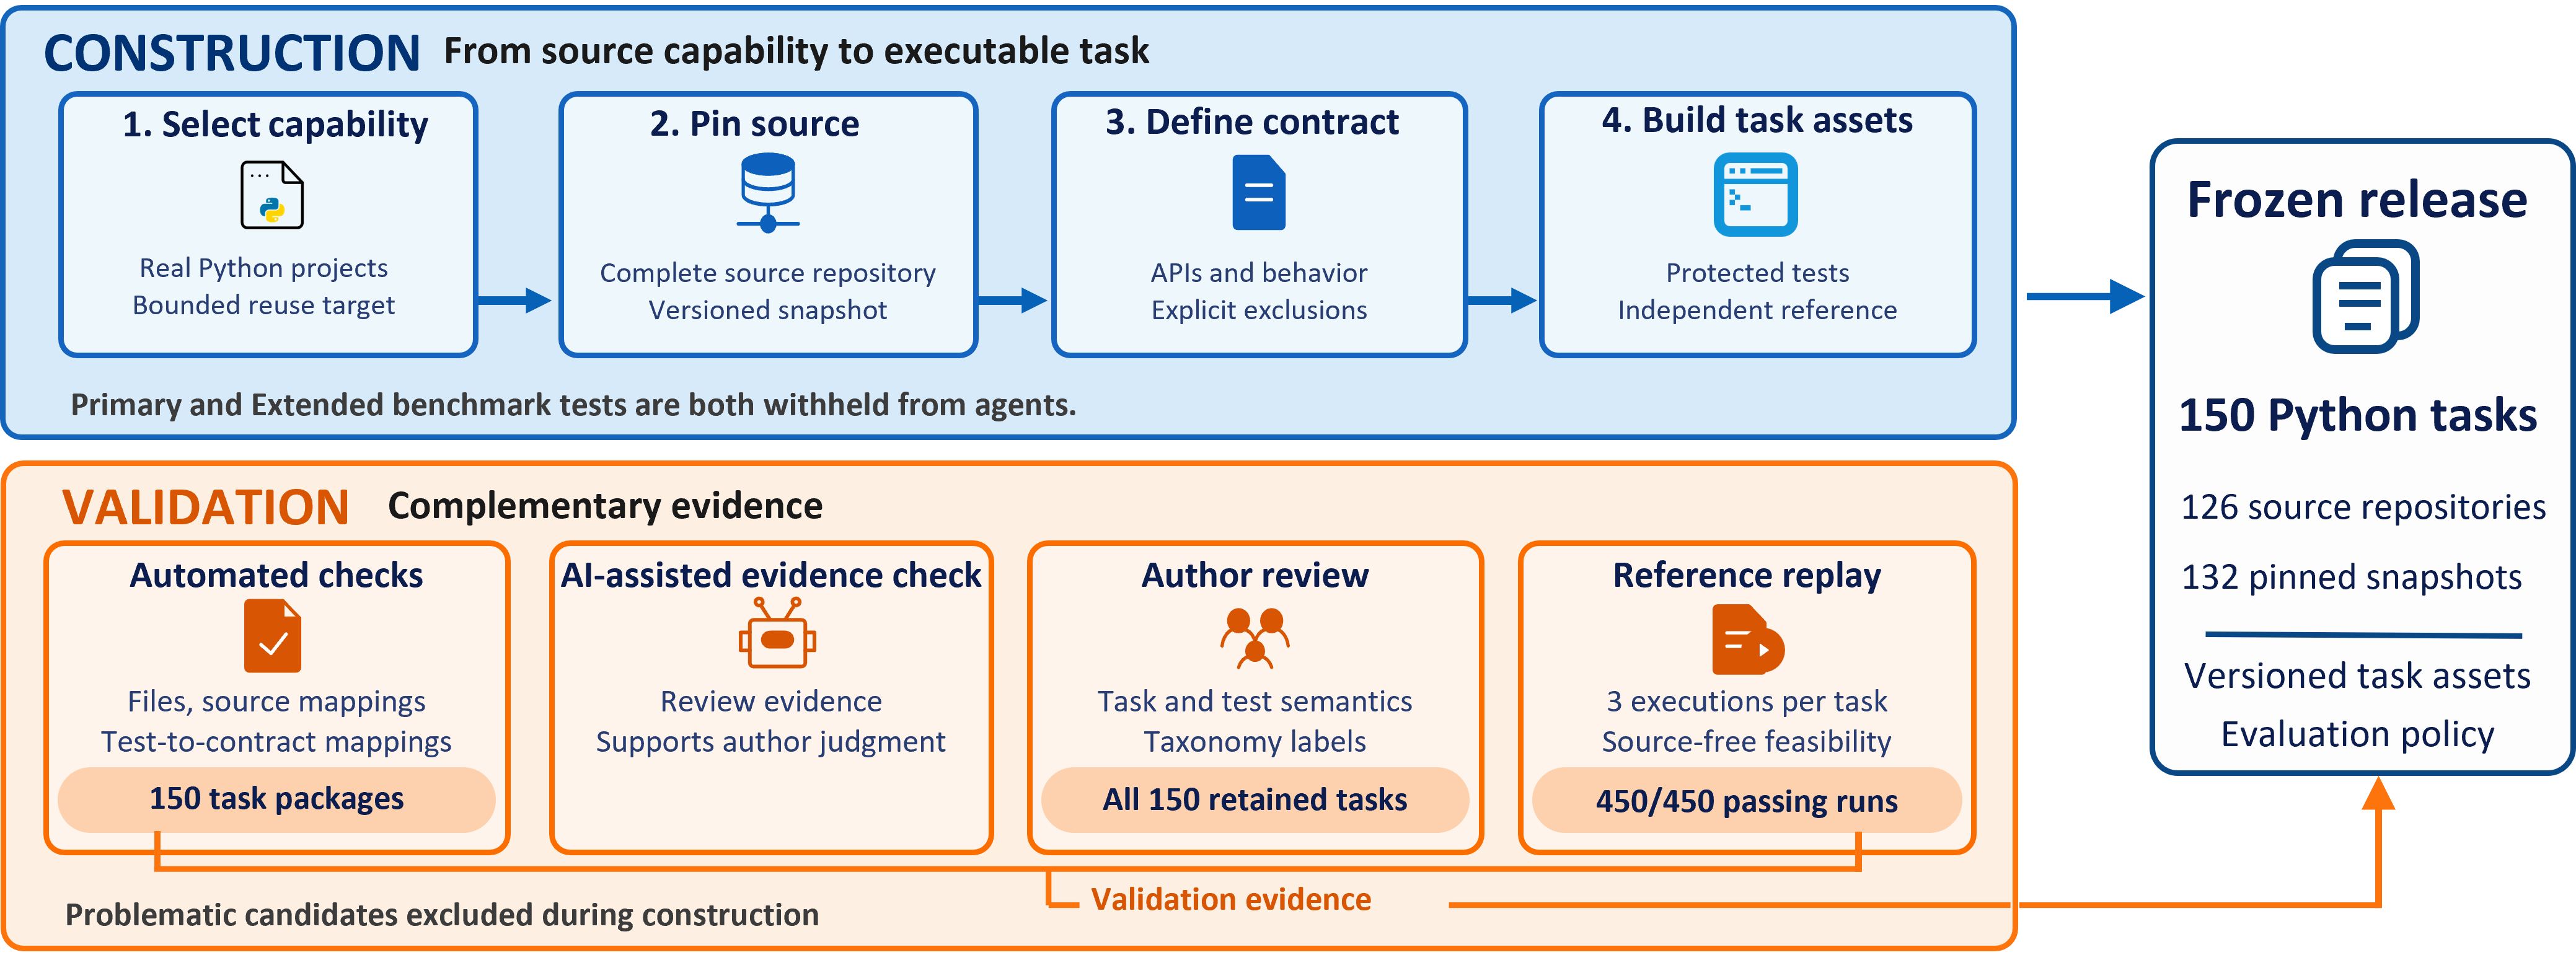
\includegraphics[width=\linewidth]{figures/fig2.png}
  \caption{Construction and validation of \flb. Construction turns a pinned
  source capability into a public contract, protected tests, and a feasible
  source-independent reference package. Validation combines automated
  consistency checks, multi-author semantic review supported by structured
  AI-assisted checks, and three successful source-free reference replays per task
  (450/450 executions).}
  \Description{The upper band shows task construction from capability selection
  and source pinning through contract definition and protected evaluation assets.
  The lower band shows structural checks, semantic review, and repeated reference
  execution before tasks enter the frozen benchmark.}
  \label{fig:construction}
\end{figure}

\subsection{Dataset Composition}
\label{sec:suite}

We characterize the 150 tasks along three complementary dimensions:
\emph{functional family} describes what capability is lifted, \emph{lift type}
describes how the requested capability relates to its upstream implementation,
and \emph{entanglement} describes which forms of project dependency must be
handled when crossing the new package boundary. These annotations describe
benchmark composition and do not affect scoring.

\paragraph{Functional coverage.}
The benchmark spans ten functional families across 126 repositories and 132
pinned source snapshots. The largest families are parsing/tokenizing/decoding
(31 tasks), registry/plugin dispatch (22), serialization/formatting/rendering
(19), configuration resolution/discovery (18), and
validation/normalization/construction (15). The remaining tasks cover workflow
and session orchestration, resource and metadata loading, algorithms and data
structures, protocol state transitions, and cache/retry policies.

\paragraph{Lift types.}
Each task receives one of three labels according to the relation between the
requested capability and its upstream implementation. \emph{Direct} tasks
preserve an identifiable upstream capability while extracting it from its
original project context. \emph{Adapted} tasks retain an identifiable capability
but require a declared change to its interface or observable behavior.
\emph{Composite} tasks combine multiple upstream capabilities or reconstruct a
workflow without a single corresponding upstream API. The benchmark contains 56
Direct, 76 Adapted, and 18 Composite tasks. These labels characterize the
requested transformation rather than the implementation strategy used by an
agent.

\paragraph{Entanglement mechanisms.}
Tasks may additionally carry multiple labels describing the dependencies that
must be accounted for during lifting. We group the underlying annotations into
four mechanisms: \emph{code dependencies}, covering internal helpers, transitive
imports, and third-party interfaces; \emph{data and state}, covering shared
models, parser state, and registries; \emph{framework mechanisms}, covering
lifecycle, dispatch, and dynamic discovery; and \emph{environment and
resources}, covering configuration, path rules, and packaged resources. These
mechanisms are non-exclusive and describe where a capability is coupled to its
host project rather than independent difficulty factors.

Figure~\ref{fig:coverage} summarizes the resulting composition. Panel~(a) shows
the ten functional families partitioned by lift type, while panel~(b) shows the
prevalence of the four entanglement mechanisms overall and within each lift
type.

\begin{figure}[tbp]
  \centering
  \begin{minipage}[c]{0.57\linewidth}
    \centering
    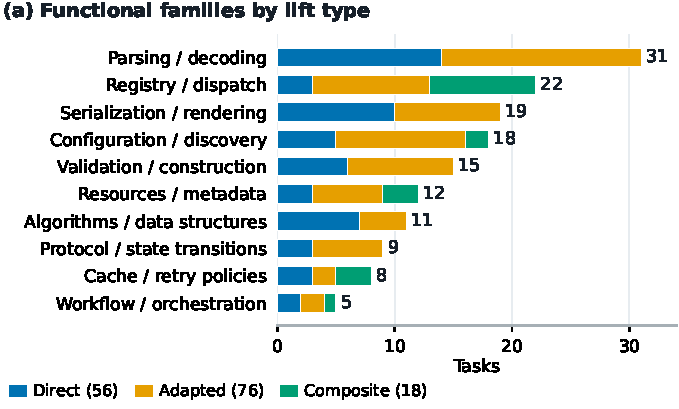
\includegraphics[width=\linewidth]{figures/fig3a_families.pdf}
  \end{minipage}
  \hfill
  \begin{minipage}[c]{0.41\linewidth}
    \centering
    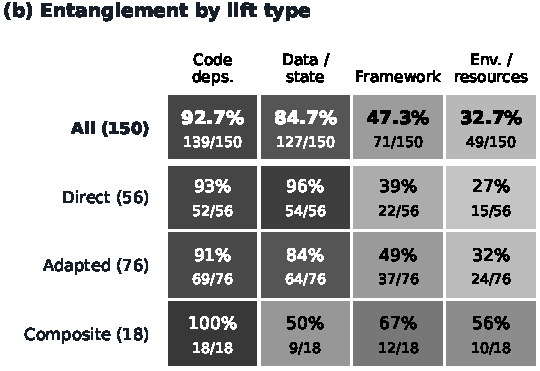
\includegraphics[width=\linewidth]{figures/fig3b_entanglement.pdf}
  \end{minipage}
  \caption{Composition of the 150-task benchmark. (a) Ten functional families
  partitioned by lift type: Direct (56), Adapted (76), and Composite (18).
  (b) Coverage of four non-exclusive entanglement mechanisms overall and within
  each lift type; cells report percentages and task counts. These annotations
  characterize benchmark composition rather than predefined difficulty.}
  \Description{Panel (a) shows ten functional families as stacked horizontal
  bars partitioned by the three lift types. Panel (b) shows a heatmap of code
  dependencies, data and state, framework mechanisms, and environment or
  resource entanglement, overall and within each lift type.}
  \label{fig:coverage}
\end{figure}

\section{Evaluation Protocol and Experimental Setup}
\label{sec:protocol}

We evaluate six model--harness configurations on the same 150 tasks under a
shared information and evaluation policy. This section specifies the evaluated
systems, functional and artifact metrics, statistical protocol, and the two
diagnostic analyses used to study repository evidence.

\subsection{Information Boundary and Agent Configurations}

We evaluate DeepSeek V4 Pro, DeepSeek V4 Flash, GPT-5.6 Luna, GLM-5.3-Flash,
Qwen3.6-35B-A3B-FP8, and GPT-OSS 120B, abbreviated as Pro, Flash, Luna, GLM,
Qwen, and OSS. All configurations use OpenHands CLI 1.16.0 with native tool
calling~\cite{wang2025openhands}. Agents receive the complete pinned source repository and public
behavioral contract, while benchmark tests, reference implementations, and
benchmark-provided source-location hints are withheld.

Every run in the main comparison and paired ablation uses a 3,600-second timeout,
a 131,072-token context window with 8,192 tokens reserved for output, and the
same maximum of 120 interaction steps. In the main comparison, Pro and Flash use
token-based context condensation; the remaining configurations use the default
OpenHands context handling. Work on agent--computer interfaces and harness
effects motivates reporting these execution choices as part of the evaluated
system~\cite{yang2024sweagent,yao2026harnessbench}. We therefore treat each
model--harness configuration as the experimental unit rather than attributing
observed differences to the base model alone.

\subsection{Functional Evaluation and Artifact Metrics}

Only the collected submission enters the evaluator environment; the source
repository is unavailable at runtime, networking is disabled, and dependencies
are fixed. Functional success follows Equation~\ref{eq:functional}. The
\textbf{Build} gate checks that the submitted package can be loaded under the
frozen evaluator environment; \textbf{Primary} and \textbf{Extended} exercise
withheld behavioral obligations from the same public contract; and
\textbf{Isolation} checks prohibited source dependencies and protected-path
access.

\paragraph{Successful-artifact characteristics.}
For a functionally passing artifact $A$ and its frozen feasible reference
$A_{\mathrm{ref}}$, we define Reference-Relative Extraction Size as
\begin{equation}
  \operatorname{RRES}(A)=
  \frac{\operatorname{PythonLOC}(A)}
       {\operatorname{PythonLOC}(A_{\mathrm{ref}})}.
  \label{eq:rres}
\end{equation}
RRES characterizes artifact size relative to one feasible reference; it does
not measure minimality.

We additionally report \emph{Copy}, the fraction of submitted Python source
matched to the source repository in normalized runs of at least three non-empty,
non-comment lines. Copy measures syntactic overlap rather than semantic
equivalence, a distinction established in code-clone
research~\cite{roy2009clones}, and can miss rewritten equivalents.
Both RRES and Copy are reported only after functional success and
are not incorporated into the functional score.

\paragraph{Execution effort.}
We report recorded assistant-step counts for all assigned tasks. Token usage
includes uncached prompt plus completion tokens for Pro and Flash, and total
tokens for Luna, GLM, Qwen, and OSS. These measurements are descriptive within
their respective accounting definitions rather than a cross-provider cost ranking.

\subsection{Comparison Scope and Statistical Analysis}

The main comparison contains one retained outcome for each of six configurations
on each of the same 150 tasks, yielding 900 model--task outcomes. All assigned
tasks remain in the denominator, including runs that produce no usable
submission. Functional correctness is determined by the frozen evaluator rather
than by the agent runner's terminal status.

We treat the resulting pass rates as observed performance of the evaluated
model--harness configurations. Because each configuration contributes one
retained outcome per task, the main comparison does not estimate run-to-run
stochastic variance.

The source-evidence ablation compares Full Source and Contract Only on the same
tasks using paired pass-rate differences, paired bootstrap confidence intervals,
and exact conditional McNemar tests~\cite{fagerland2013mcnemar}, with Holm
correction across configurations~\cite{holm1979multiple}. Intervals use
100{,}000 paired task-bootstrap resamples and describe variation across task
pairs rather than repeated agent runs.

For successful-artifact comparisons, we retain tasks with successful artifacts
from at least two configurations and fit task fixed-effects models:
\begin{equation}
\begin{aligned}
  \log_2\!\left(\operatorname{RRES}_{t,m}\right)
    &= \alpha_t^{\mathrm{RRES}} + \beta_m^{\mathrm{RRES}}
       + \epsilon_{t,m}^{\mathrm{RRES}}, \\
  \operatorname{Copy}_{t,m}
    &= \alpha_t^{\mathrm{Copy}} + \beta_m^{\mathrm{Copy}}
       + \epsilon_{t,m}^{\mathrm{Copy}},
\end{aligned}
\label{eq:adjusted-footprint}
\end{equation}
with $\sum_m\beta_m^{\mathrm{RRES}}=\sum_m\beta_m^{\mathrm{Copy}}=0$.
Here $t$ indexes tasks and $m$ indexes configurations. Ordinary least squares
gives each successful artifact equal weight. We report the task-adjusted RRES
ratio $2^{\beta_m^{\mathrm{RRES}}}$ and the Copy difference
$100\beta_m^{\mathrm{Copy}}$ in percentage points. Their reference centers,
$1\times$ and 0 pp, represent the sum-to-zero center of configuration effects;
the RRES ratio is not an adjusted median or a raw size ratio to the reference
implementation.

Pointwise 95\% percentile intervals use 10{,}000 accepted task-cluster bootstrap
resamples~\cite{field2007cluster}, retaining all successful artifacts of each sampled task and refitting
and centering both models on every resample. We check that the six-configuration
co-success graph remains connected; a disconnected draw would be rejected and
redrawn. Sensitivity analyses give each artifact weight $1/k_t$, where $k_t$ is
the number of successful configurations on task $t$, or resample whole source
repositories while retaining artifact weights from the main analysis. Each uses
10{,}000 accepted resamples; no disconnected draws occurred in any scheme.
These intervals describe variation across task or repository clusters, not
repeated agent runs. The analysis is descriptive and conditional on success;
it does not estimate causal configuration effects or a global quality ranking.

\subsection{Paired Source-Evidence Ablation}
\label{sec:source-ablation-protocol}

The main benchmark intentionally provides the intact source repository because
feature lifting studies reconstruction from existing implementation evidence. To
test whether that evidence materially affects success, we conduct a paired
ablation that removes the repository while keeping the requested behavior fixed.

We select a fixed 40-task subset from 38 repositories, containing 15 Direct,
20 Adapted, and 5 Composite tasks. The subset was stratified by lift type and
frozen before inspecting ablation outcomes. GPT-5.6 Luna,
DeepSeek V4 Pro, and Qwen3.6-35B-A3B-FP8 are each evaluated under two conditions
on the same tasks, yielding 240 retained outcomes. These are new paired runs
rather than reused outcomes from the main comparison.

In the \emph{Full Source} condition, the agent receives the complete pinned
repository together with the public behavioral contract. In \emph{Contract
Only}, the repository is omitted while the same contract and permitted
dependency information are retained; retrieving the original project from the
network, installed packages, or caches is prohibited. Benchmark tests, reference
implementations, and source-location hints remain hidden in both conditions. The
intervention therefore removes repository evidence as a whole, including source
code, upstream tests, documentation, and packaged resources, rather than
isolating source-code text alone.

Within each configuration, the paired conditions use the same model--harness
settings and source-free evaluator. The Pro configuration in this ablation does
not apply context compression. We compare functional success using
paired pass-rate differences, paired bootstrap confidence intervals, and exact
McNemar tests with Holm correction across the three configurations. Missing
submissions remain functional failures. We make one fresh attempt for each of
18 Pro Contract-Only runs initially recorded as timeouts without a submission.
Six produce evaluable artifacts and replace their original outcomes under a
predefined earliest-eligible-attempt rule, regardless of functional success;
the other 12 retain their original failed outcomes. All attempts are preserved.

\subsection{Trace-Based Source-Exposure Measurement}
\label{sec:source-exposure-protocol}

To distinguish source availability from observable source use, we analyze the
900 saved trajectories from the main comparison without rerunning agents. For
each task, we statically map its declared source entrypoints to files in the
pinned repository. This resolves 607 of 641 declared entrypoints; at least one
entrypoint is resolved for 145 of the 150 tasks.

We call an event a \emph{confirmed source read} when a successful tool read
returns content matching at least two adjacent normalized source lines from a
mapped file. Filename mentions, unsuccessful reads, and traceback text do not
qualify. Unresolved mappings remain unconfirmed rather than being treated as
absence of source inspection. This measure therefore captures observable
exposure to entrypoint-associated source-file content, not whether the agent
located the complete implementation, followed all supporting dependencies, or
understood the returned code. We use it as a diagnostic of whether behavioral
failures can persist after relevant source content has already been observed.

\subsection{Retrospective Execution-Effort Analysis}
\label{sec:execution-effort-protocol}

We analyze the retained main-comparison runs without invoking the agents again.
For outcome-level expenditure, we sum verified input and output tokens over
model calls, including cache-hit input once. Runs with missing call usage are
unavailable for this analysis; they are not assigned zero tokens. This total-token
accounting differs from the uncached-input accounting for Pro and Flash in
Table~\ref{tab:main} and does not measure cross-provider prices or computation.

For trajectory-level analysis, we use saved reconstructions at tool-completion
boundaries, evaluated with the four functional gates. We identify the first
\emph{observed passing checkpoint} among these reconstructed versions. Let
$T_r^{\mathrm{obs}}$ denote cumulative tokens at this checkpoint and $T_r$ the
run total. The post-sufficiency fraction is
$\mathrm{PSF}_r=(T_r-T_r^{\mathrm{obs}})/T_r$.
We also count subsequent model calls, excluding the call that produced the
passing checkpoint. Both measures use the same conservative subset of final
successes with complete token ledgers, exact call alignment, evaluated checkpoint
chains, and matching reconstructed and re-evaluated final submissions. Values
are summarized per run before aggregation. We do not claim to recover every
transient filesystem state or infer a stopping signal available to the agent.

\section{Benchmark Results}
\label{sec:results}

We organize the results around five questions: \textbf{RQ1} measures overall
feature-lifting capability; \textbf{RQ2} examines execution effort across outcomes
and after an observed passing artifact; \textbf{RQ3} diagnoses functional failures
and their persistence after source-file exposure; \textbf{RQ4} tests the effect
of repository evidence through paired ablation; and \textbf{RQ5} characterizes
the implementation footprint of functionally successful artifacts.

\subsection{RQ1: How Capable Are Current Coding Agents at Feature Lifting?}
\label{sec:rq1}

Table~\ref{tab:main} reports the main comparison over the same 150 tasks for all
six configurations. DeepSeek V4 Pro achieves the highest observed functional
success, passing 115/150 tasks (76.7\%), followed by Flash at 108/150 (72.0\%)
and Luna at 102/150 (68.0\%). GLM, Qwen, and OSS pass 68 (45.3\%), 63 (42.0\%),
and 36 (24.0\%) tasks, respectively.

These results show substantial but incomplete feature-lifting capability. Even
the strongest configuration fails 35 of the 150 frozen tasks under the same
source-access and evaluation policy. Because each model--task cell contains one
retained run, the values describe observed performance of the evaluated
model--harness configurations rather than run-to-run success probabilities.

% BEGIN GENERATED TABLE: main
\begin{table}[tbp]
  \caption{Main comparison on the common 150-task benchmark. Artifact
  characteristics are reported only for functionally successful submissions.}
  \label{tab:main}

  \centering
  \footnotesize
  \setlength{\tabcolsep}{2.2pt}
  \renewcommand{\arraystretch}{1.12}

  \begin{tabularx}{\linewidth}{@{}Xr rrr rrr rr rr@{}}
    \toprule

    &
    \multicolumn{1}{c}{Correctness} &
    \multicolumn{3}{c}{RRES} &
    \multicolumn{3}{c}{Copy} &
    \multicolumn{2}{c}{Steps} &
    \multicolumn{2}{c}{Tokens ($10^3$)} \\

    \cmidrule(lr){2-2}
    \cmidrule(lr){3-5}
    \cmidrule(lr){6-8}
    \cmidrule(lr){9-10}
    \cmidrule(lr){11-12}

    Configuration
      & \shortstack{Pass@1\\$n$ (\%)}
      & Mean
      & Median
      & $[Q_1,Q_3]$
      & Mean
      & Median
      & $[Q_1,Q_3]$
      & Median
      & P90
      & Median
      & P90 \\

    \midrule
    DeepSeek V4 Pro$^{\dagger}$ & \textbf{115 (76.7)} & 1.781 & 0.993 & [0.769, 1.290] & 0.777 & 0.957 & [0.716, 0.987] & 41.5 & 80.1 & 88.0 & 225.3 \\
    DeepSeek V4 Flash$^{\dagger}$ & 108 (72.0) & 1.730 & 0.998 & [0.893, 1.221] & 0.810 & 0.968 & [0.839, 0.990] & 63.0 & 116.2 & 123.6 & 269.5 \\
    GPT-5.6 Luna$^{\ddagger}$ & 102 (68.0) & 0.953 & 0.815 & [0.310, 1.002] & 0.415 & 0.164 & [0.048, 0.967] & 35.5 & 74.4 & 1483.7 & 11349.4 \\
    GLM-5.3-Flash$^{\ddagger}$ & 68 (45.3) & 2.473 & 1.013 & [0.917, 1.158] & 0.843 & 0.947 & [0.811, 0.979] & 85.5 & 127.0 & 7018.5 & 18791.9 \\
    Qwen3.6-35B-A3B-FP8$^{\ddagger}$ & 63 (42.0) & 1.556 & 0.975 & [0.650, 1.228] & 0.645 & 0.757 & [0.326, 0.972] & 41.5 & 106.6 & 1818.6 & 5521.0 \\
    GPT-OSS 120B$^{\ddagger}$ & 36 (24.0) & 1.176 & 0.983 & [0.292, 1.648] & 0.305 & 0.180 & [0.007, 0.530] & 19.0 & 61.1 & 526.0 & 1877.3 \\


    \bottomrule
  \end{tabularx}

  \par\smallskip
  \begin{minipage}{\linewidth}
    \footnotesize
    Pass@1 uses all 150 assigned tasks; RRES and Copy use only functionally
    passing artifacts. Steps use all assigned runs. $^{\dagger}$ reports
    uncached prompt plus completion tokens; $^{\ddagger}$ reports total
    tokens. These accounting schemes are not directly comparable.
  \end{minipage}

\end{table}
% END GENERATED TABLE: main


\paragraph{Observed variation across task structures.}
Table~\ref{tab:structure} reports pass rates within the three lift types
and four overlapping entanglement-mechanism groups. Pro, Flash, and Luna have lower
observed pass rates on Adapted and Composite tasks than on Direct tasks.
These descriptive comparisons do not isolate a causal difficulty effect:
category membership co-varies with other task properties, and the Composite
group contains only 18 tasks.


% BEGIN RESULTS EVIDENCE: structure
\begin{table}[tbp]
  \centering
  \footnotesize
  \caption{Observed functional pass rates (\%) by task structure.}
  \label{tab:structure}
  \begin{tabularx}{\linewidth}{@{}Xrrrrrrr@{}}
    \toprule
    Category & $n$ & Pro & Flash & Luna & GLM & Qwen & OSS \\
    \midrule
    Direct & 56 & 91.1 & 89.3 & 80.4 & 71.4 & 55.4 & 28.6 \\
    Adapted & 76 & 72.4 & 67.1 & 65.8 & 31.6 & 35.5 & 21.1 \\
    Composite & 18 & 50.0 & 38.9 & 38.9 & 22.2 & 27.8 & 22.2 \\
    \midrule
    Code dependencies & 139 & 79.9 & 73.4 & 69.1 & 46.0 & 42.4 & 22.3 \\
    Data and state & 127 & 80.3 & 75.6 & 71.7 & 48.0 & 44.1 & 23.6 \\
    Framework mechanisms & 71 & 78.9 & 73.2 & 66.2 & 40.8 & 43.7 & 16.9 \\
    Environment and resources & 49 & 75.5 & 71.4 & 63.3 & 32.7 & 34.7 & 24.5 \\
    \bottomrule
  \end{tabularx}
  \par\smallskip\begin{minipage}{\linewidth}\scriptsize
  $n$ is the row denominator. Lift types partition the tasks; mechanism groups overlap.
  \end{minipage}
\end{table}
% END RESULTS EVIDENCE: structure

\subsection{RQ2: How Much Execution Effort Do Agents Expend on Feature Lifting?}
\label{sec:rq2}

Final pass rates do not reveal how effort differs across outcomes or when a
sufficient artifact first appears. We therefore examine outcome-level token
expenditure and execution after an observed passing checkpoint separately.

\paragraph{Token expenditure varies across outcomes.}
Table~\ref{tab:execution-effort} reports outcome-conditioned expenditure under
a common total-token definition. Failed runs have higher median expenditure
than successful runs for Pro, Flash, and OSS, whereas Qwen shows the opposite
pattern. For example, Pro's medians are 2.24 million tokens for successes and
2.71 million for failures; Qwen's are 2.13 million and 1.30 million, respectively.
These comparisons concern different task sets and do not imply that greater
expenditure causes success or failure. Historical per-call usage is unavailable
for Luna and GLM, so their conditional token distributions are not reported.

% BEGIN RESULTS EVIDENCE: execution-effort
\begin{table}[tbp]
  \centering
  \footnotesize
  \caption{Token expenditure by final outcome.}
  \label{tab:execution-effort}
  \begin{tabularx}{\linewidth}{@{}Xrlrl@{}}
    \toprule
    & \multicolumn{2}{c}{Successful runs} & \multicolumn{2}{c}{Failed runs} \\
    \cmidrule(lr){2-3}\cmidrule(lr){4-5}
    Configuration & $n/N$ & Median [IQR] & $n/N$ & Median [IQR] \\
    \midrule
    Pro & 115/115 & 2.24 [1.46, 3.88] & 34/35 & 2.71 [1.79, 4.67] \\
    Flash & 108/108 & 4.01 [2.20, 7.08] & 42/42 & 4.72 [3.16, 8.46] \\
    Luna & 0/102 & -- & 0/48 & -- \\
    GLM & 0/68 & -- & 0/82 & -- \\
    Qwen & 63/63 & 2.13 [1.59, 3.24] & 83/87 & 1.30 [0.25, 3.28] \\
    OSS & 33/36 & 0.38 [0.23, 0.95] & 112/114 & 0.55 [0.30, 1.09] \\
    \bottomrule
  \end{tabularx}
  \par\smallskip\begin{minipage}{\linewidth}\scriptsize
  Tokens are input plus output, including cached input, in millions. $n/N$ denotes usable records over assigned runs with that outcome.
  \end{minipage}
\end{table}
% END RESULTS EVIDENCE: execution-effort

\paragraph{Execution continues after an observed passing artifact.}
The jointly measurable successful subsets contain 89/115 Pro, 75/108 Flash,
5/63 Qwen, and 25/36 OSS runs. Figure~\ref{fig:execution-effort} shows their
post-checkpoint distributions. Median PSF is 67.3\% for Pro and 72.3\% for
Flash, accompanied by medians of 19 and 29 subsequent model calls. Qwen and
OSS have median PSF values of 53.7\% and 37.1\%, with 11 and 4 subsequent
calls; Qwen's five recoverable runs are a small descriptive subset. The samples
differ across configurations and do not support an adjusted efficiency ranking.
Points represent tasks; boxes summarize quartiles with 1.5-IQR whiskers, while
Qwen's small sample is shown as individual points and its median.

\begin{figure}[tbp]
  \centering
  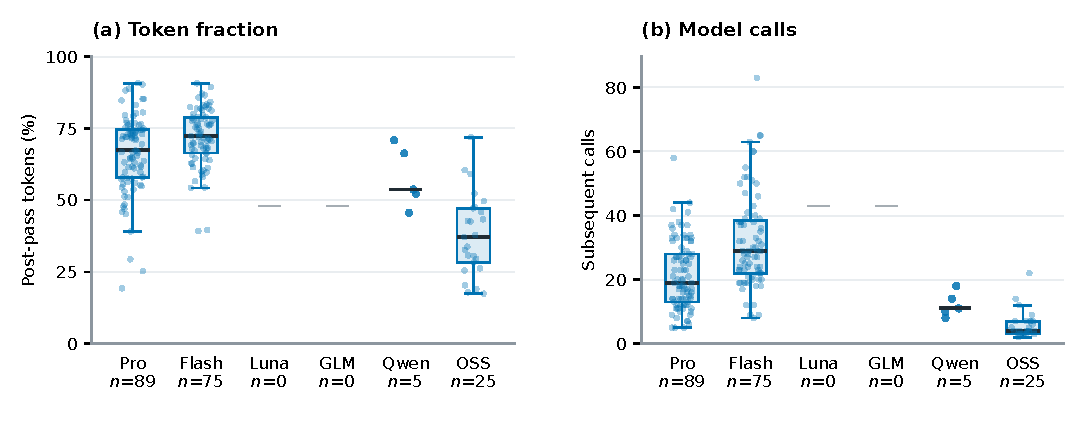
\includegraphics[width=\linewidth]{figures/fig_execution_effort.pdf}
  \caption{Execution after the first reconstructed passing checkpoint: (a) token fraction; (b) subsequent model calls.}
  \Description{Two panels show post-checkpoint token fractions and subsequent model calls for Pro, Flash, Qwen, and OSS. Luna and GLM have no jointly measurable sample.}
  \label{fig:execution-effort}
\end{figure}

Using the first checkpoint after which all remaining reconstructed checkpoints
pass changes the median token fractions to 67.3\%, 71.1\%, 53.7\%, and
37.1\%, respectively, on the same samples. The observed continuation therefore
is not explained solely by temporarily passing and then repairing regressions.
It also need not be unproductive: in an inspected Pro JSONPath trajectory,
subsequent actions run tests, inspect dependencies, and clean generated files
without changing the evaluated artifact. Repeated context consumption matters:
under the uncached-input accounting used in Table~\ref{tab:main}, median
post-checkpoint fractions for the same Pro and Flash samples are 33.7\% and
41.5\%. These observations characterize continued execution, not a directly
recoverable saving in tokens, cost, or computation.

\subsection{RQ3: Where Do Functional Failures First Emerge, and Do They Persist After Observed Source-File Exposure?}
\label{sec:rq3}

We first locate the observed boundary at which each unsuccessful run ceases to
satisfy the evaluation protocol. We classify each run as Pass, no usable
submission, or by its first failed evaluator gate in the sequence
Build--Primary--Extended--Isolation. This classification identifies where
failure becomes observable; it does not by itself establish the underlying
cause.

Figure~\ref{fig:failures} shows a clear pattern among the strongest
configurations. Pro and Flash produce usable submissions for all 150 tasks and
have no Build-first failures. Of their 77 combined unsuccessful runs, 76 first
fail at Primary or Extended, and only one first fails at Isolation. Thus, once
these configurations deliver a package, the dominant remaining boundary is
behavioral preservation rather than package production or loading.

Weaker configurations exhibit a broader mixture of failure modes. GLM and Qwen
produce no usable submission for 38 and 25 tasks, respectively, while OSS
usually delivers an artifact but has 18 Build-first and 93
Primary/Extended-first failures. Low overall success therefore need not reflect
the same operational bottleneck across configurations.

\begin{figure}[tbp]
  \centering
  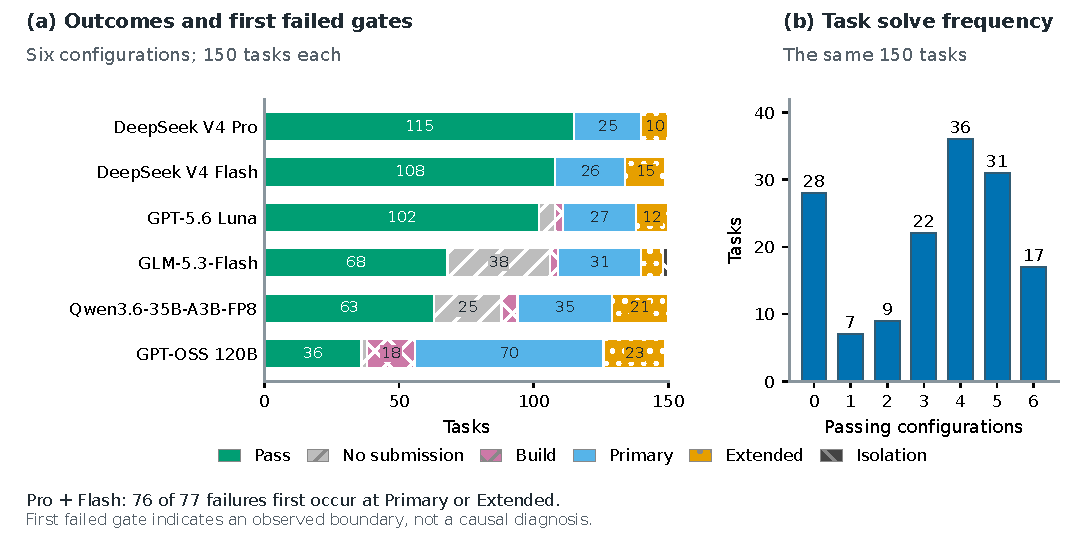
\includegraphics[width=\linewidth]{figures/fig4.pdf}
  \caption{Functional outcomes by configuration, partitioned into success, no submission, and first failed evaluator gate.}
  \Description{Horizontal stacked bars show Pass, no usable submission,
  Build-first, Primary-first, Extended-first, and Isolation-first outcomes for
  six configurations over 150 tasks each.}
  \label{fig:failures}
\end{figure}

\paragraph{Behavioral failures often persist after source exposure.}
A behavioral-first failure could arise simply because the agent never inspected
implementation evidence associated with the requested capability. The saved
trajectories show that this explanation is insufficient for many runs. Among the
303 Primary/Extended-first failures across all six configurations, 241 (79.5\%)
contain a confirmed read returning content from an entrypoint-associated source
file (Table~\ref{tab:source-exposure}). The median first confirmed read among these runs occurs at tool action
five. For Pro and Flash alone, 63 of their 76 behavioral-first failures contain
such exposure.

These observations show that opening entrypoint-associated source files is not
sufficient for successful feature lifting. A confirmed read does not establish
that the agent recovered all supporting dependencies or understood the complete
behavioral closure, so the result should not be interpreted as a causal diagnosis
of why individual runs fail. It nevertheless rules out a simple account in
which most behavioral failures occur before any associated source content is
observed.

% BEGIN VERIFIED SOURCE EXPOSURE TABLE
\begin{table}[tbp]
  \centering
    \caption{Source exposure by final outcome.}
    \label{tab:source-exposure}

    \centering
    \footnotesize

    \begin{tabular}{@{}lrrr@{}}
      \toprule
      Outcome
        & Runs
        & \shortstack{Confirmed read\\$n/N$ (\%)}
        & \shortstack{Median first\\read step} \\
      \midrule
      Pass & 492 & 363/492 (73.8) & 5 \\
      Behavioral-first & 303 & \textbf{241/303 (79.5)} & 5 \\
      Delivery/build & 101 & 51/101 (50.5) & 5 \\
      Isolation-first & 4 & 4/4 (100.0) & 10.5 \\

      \bottomrule
    \end{tabular}

    \par\smallskip
    {\scriptsize
    Read-step medians are conditional on confirmed source reads.
    }
\end{table}
% END VERIFIED SOURCE EXPOSURE TABLE

\paragraph{Behavior drift dominates the reviewed failures.}
We analyze a reviewed set of 228 source-exposed behavioral failures.
Multiple coauthors reviewed the failure classifications against the public
contracts, submitted implementations, and evaluation logs.
Each failure has one primary category.
Figure~\ref{fig:failure-analysis} compares category composition within each
configuration; Table~\ref{tab:failure-analysis} defines the taxonomy and
reports pooled counts and percentages.
Of these, 201 (88.2\%) exhibit behavior drift: the required API exists, but its
observable behavior differs from the public contract. Behavior drift is also
the largest category within every configuration.
This distribution suggests that preserving behavior through the reconstructed
API is the dominant remaining issue within this reviewed set, even after an
entrypoint-associated source file has been read.

\begin{figure}[tbp]
  \centering
  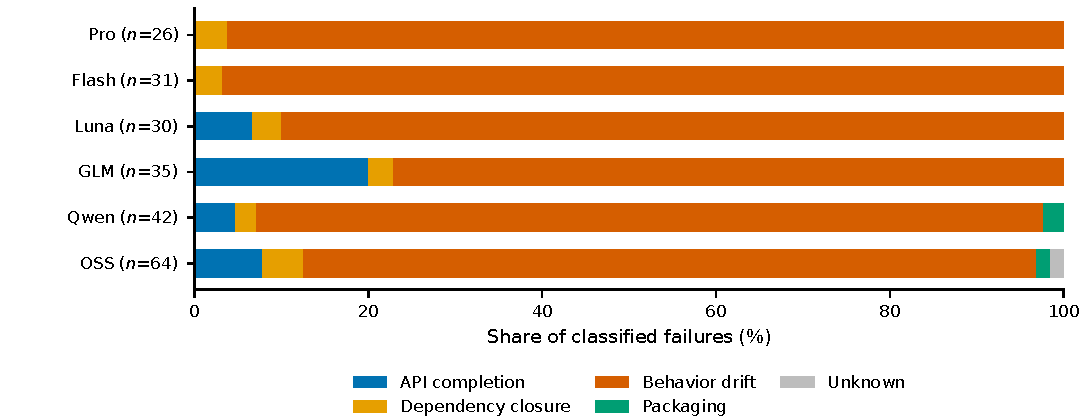
\includegraphics[width=\linewidth]{figures/fig8_failure_analysis.pdf}
  \caption{Within-configuration composition of reviewed source-exposed behavioral failures.}
  \Description{Six horizontal stacked bars show the distribution of API
  completion, dependency closure, behavior drift, packaging, and unknown
  categories. Behavior drift is the largest category for every configuration.}
  \label{fig:failure-analysis}
\end{figure}


% BEGIN RESULTS EVIDENCE: failure-analysis
\begin{table}[tbp]
  \centering
  \footnotesize
  \caption{Failure taxonomy and pooled counts after confirmed source reading.}
  \label{tab:failure-analysis}
  \begin{tabularx}{\linewidth}{@{}p{0.23\linewidth}Xr@{}}
    \toprule
    Category & Observed gap & $n$ (\%) \\
    \midrule
    \textbf{Behavior drift} & Required API exists, but observable behavior differs from the contract. & \textbf{201 (88.2)} \\
    API completion & Required export, member, or API path is missing. & 16 (7.0) \\
    Dependency closure & A required helper, resource, registry, or dependency is absent. & 8 (3.5) \\
    Packaging & Implementation is present but not exposed through the standalone package. & 2 (0.9) \\
    Localization & Trajectory and submission indicate the wrong implementation region. & 0 (0.0) \\
    Unknown & Available evidence does not distinguish a primary category. & 1 (0.4) \\
    \bottomrule
  \end{tabularx}
  \par\smallskip\begin{minipage}{\linewidth}\scriptsize
  $N=228$ reviewed failures; one primary category per failure.
  \end{minipage}
\end{table}
% END RESULTS EVIDENCE: failure-analysis

\subsection{RQ4: Does Repository Evidence Improve Behavioral Reconstruction?}
\label{sec:rq4}
\label{sec:source-ablation-results}

Repository evidence substantially improves functional success on the paired
40-task ablation (Figure~\ref{fig:source-evidence}). GPT-5.6 Luna passes 23/40
tasks with Full Source versus 9/40 with Contract Only, a gain of 35.0 percentage
points. Qwen passes 12/40 versus 1/40, a gain of 27.5 points. Both paired
differences remain significant after Holm correction ($p=0.00515$ for each).
Pro passes 25/40 tasks with Full Source and 7/40 with Contract Only, a gain of
45.0 percentage points. In the latter condition, 12 runs fail to complete during
long-context execution without context compression and return no submission.
These are unsuccessful attempts under the evaluated configuration and remain
in the denominator. Pro's result therefore reflects both behavioral
reconstruction and the configuration's ability to complete long-context runs.

\begin{figure}[tbp]
  \centering
  \begin{minipage}[t]{0.55\linewidth}
    \centering
    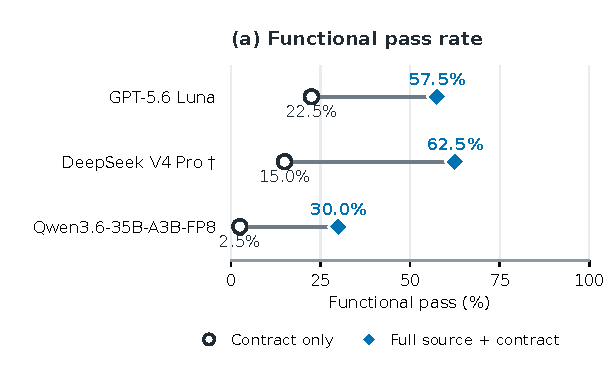
\includegraphics[width=\linewidth]{figures/fig5a_pass_rate.pdf}
  \end{minipage}
  \hfill
  \begin{minipage}[t]{0.42\linewidth}
    \centering
    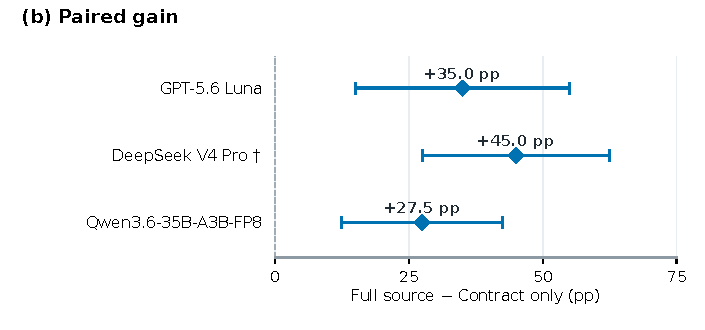
\includegraphics[width=\linewidth]{figures/fig5b_paired_gain.pdf}
  \end{minipage}
  \caption{Paired source-evidence ablation: (a) functional pass rates with Full Source and Contract Only; (b) paired pass-rate differences.}
  \Description{Two panels compare Full Source and Contract Only for GPT-5.6
  Luna, DeepSeek V4 Pro, and Qwen. Luna and Qwen have substantially higher pass
  rates with repository evidence. Pro also has a large difference, with
  12 long-context non-completions retained as Contract-Only failures.}
  \label{fig:source-evidence}
\end{figure}

% BEGIN RESULTS EVIDENCE: paired-ablation
\begin{table}[tbp]
  \centering
  \footnotesize
  \caption{Exact paired source-evidence ablation results on 40 tasks per configuration.}
  \label{tab:paired-ablation}
  \begin{tabularx}{\linewidth}{@{}Xrrrrrrr@{}}
    \toprule
    Configuration & \shortstack{Full\\pass} & \shortstack{Contract\\pass} & \shortstack{Full-\\only} & \shortstack{Contract-\\only} & \shortstack{$\Delta$\\(pp)} & \shortstack{95\%\\CI} & $p_{\mathrm{Holm}}$ \\
    \midrule
    GPT-5.6 Luna & 23/40 & 9/40 & 17 & 3 & 35.0 & [15.0, 55.0] & $5.15\times10^{-3}$ \\
    DeepSeek V4 Pro & 25/40 & 7/40 & 19 & 1 & 45.0 & [27.5, 62.5] & $1.20\times10^{-4}$ \\
    Qwen3.6-35B-A3B-FP8 & 12/40 & 1/40 & 12 & 1 & 27.5 & [12.5, 42.5] & $5.15\times10^{-3}$ \\
    \bottomrule
  \end{tabularx}
  \par\smallskip\begin{minipage}{\linewidth}\scriptsize
  Full-only and Contract-only count discordant pairs. $\Delta$: Full minus Contract (pp); CI: paired task-bootstrap interval; $p_{\mathrm{Holm}}$: Holm-adjusted exact McNemar test.
  \end{minipage}
\end{table}
% END RESULTS EVIDENCE: paired-ablation

\paragraph{The gain reflects behavioral reconstruction, not merely delivery.}
For both Luna and Qwen, every task that succeeds only under Full Source has a
Contract-Only counterpart that still produces an artifact but fails a behavioral
gate. Luna has 17 such Full-only successes and Qwen has 12; the corresponding
Contract-only counts are three and one (Table~\ref{tab:paired-ablation}). Repository evidence
therefore helps agents satisfy behavioral obligations that are missed even when
Contract Only already yields a deliverable package.

The benefit is substantial but incomplete. With Full Source available, Luna and
Qwen still exhibit behavioral-first failures, showing that access to an existing
implementation does not guarantee successful reconstruction across the new
package boundary. Because the intervention removes the repository as a whole,
these results establish the value of repository evidence---including source
code, upstream tests, documentation, and resources---rather than the isolated
causal contribution of source-code text.

\subsection{RQ5: How Do Successful Lifted Artifacts Differ in Implementation Footprint?}
\label{sec:rq5}

Table~\ref{tab:main} summarizes footprint over each configuration's successful
artifacts, but those marginal summaries involve different task sets. To compare
successful artifacts within tasks without choosing a reference configuration or
requiring all six configurations to succeed, we restrict the adjusted analysis
to 115 tasks with successful artifacts from at least two configurations,
yielding 485 successful artifacts. This excludes seven singleton successes
from the 492 successful outcomes. Included observations range from 35 for OSS
to 113 for Pro (Table~\ref{tab:matched-footprint}); the sample spans 97
repositories and includes 52 Direct, 55 Adapted, and eight Composite tasks.

Figure~\ref{fig:matched-footprint} and Table~\ref{tab:matched-footprint}
show distinct task-adjusted footprint profiles under
Equation~\ref{eq:adjusted-footprint}. Luna and OSS have estimated RRES ratios
of approximately 0.612 relative to the configuration-effect center, with 95\%
intervals of [0.537, 0.693] and [0.462, 0.767], respectively. Their adjusted
Copy differences are $-20.64$ pp and $-24.00$ pp. Pro, Flash, and GLM have
estimates above the center on both measures. Qwen has an RRES ratio of 1.109
[1.016, 1.227], while its Copy difference of $-1.79$ pp has an interval
spanning zero [$-5.89$, $+2.45$]. The reference center is symmetric across
configurations; it does not designate Pro or the benchmark reference package
as a baseline configuration. The dashed lines in
Figure~\ref{fig:matched-footprint} mark these centers; error bars show the
pointwise 95\% task-bootstrap intervals defined in our analysis protocol.

\begin{figure}[tbp]
  \centering
  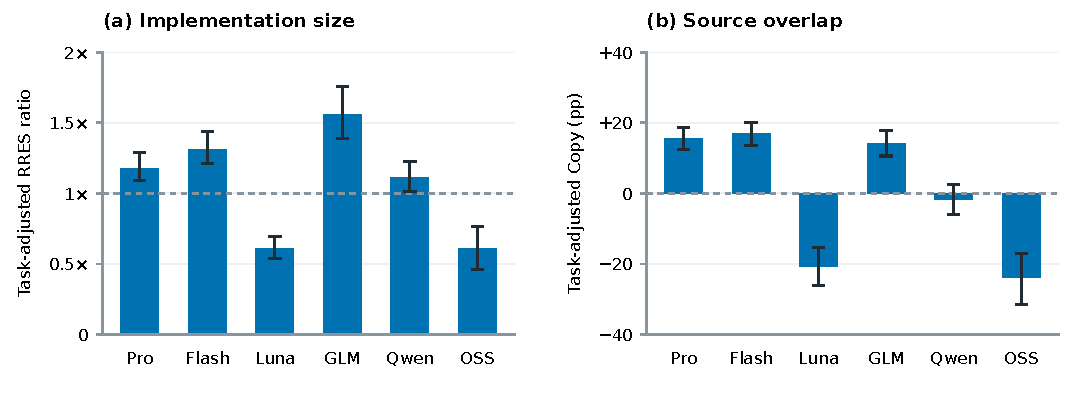
\includegraphics[width=\linewidth]{figures/fig7_matched_footprint.pdf}
  \caption{Task-adjusted successful-artifact footprints: (a) RRES ratios; (b) Copy differences in percentage points.}
  \Description{Two vertical bar charts compare Pro, Flash, Luna, GLM, Qwen,
  and OSS. The left panel shows task-adjusted implementation-size ratios with
  a reference line at one; the right shows source-overlap differences with a
  reference line at zero percentage points. Luna and OSS are below both
  centers; Qwen's source-overlap interval crosses zero. Each bar has a 95 percent
  task-bootstrap interval.}
  \label{fig:matched-footprint}
\end{figure}

\paragraph{Sensitivity to weighting and repository dependence.}
Giving each task total weight one preserves the direction of every
configuration's point estimate on both measures. Relative changes in the
estimated RRES ratios are at most 4.71\%, and changes in Copy are at most
0.78 pp. The RRES ordering of Luna and OSS reverses under this weighting,
so their near-equal point estimates do not support an ordering between them.
Repository-cluster bootstrap intervals give the same qualitative relation to
the reference centers as the main intervals, including Qwen's Copy interval
spanning zero. These checks support the footprint profiles, not a complete
pairwise ranking; overlap of two displayed intervals is not a test of their
pairwise difference.

RRES and Copy capture distinct properties: implementation size relative to a
feasible reference and detected textual overlap with the donor repository.
Neither measures minimality, maintainability, or semantic superiority.
The analysis characterizes successful artifacts only and does not extrapolate
footprint behavior to tasks on which a configuration fails.

% BEGIN RESULTS EVIDENCE: matched-footprint
\begin{table}[tbp]
  \centering
  \footnotesize
  \caption{Task-adjusted implementation footprints among successful artifacts.}
  \label{tab:matched-footprint}
  \begin{tabularx}{\linewidth}{@{}Xrrr@{}}
    \toprule
    Configuration & \shortstack{Included\\success $n$} & \shortstack{Adjusted RRES ratio\\{[95\% CI]}} & \shortstack{Adjusted Copy, pp\\{[95\% CI]}} \\
    \midrule
    Pro & 113 & 1.178 [1.088, 1.288] & $+15.42$ [$+12.35$, $+18.56$] \\
    Flash & 107 & 1.314 [1.212, 1.439] & $+16.81$ [$+13.61$, $+20.17$] \\
    Luna & 99 & 0.612 [0.537, 0.693] & $-20.64$ [$-26.07$, $-15.28$] \\
    GLM & 68 & 1.555 [1.387, 1.754] & $+14.20$ [$+10.57$, $+17.73$] \\
    Qwen & 63 & 1.109 [1.016, 1.227] & $-1.79$ [$-5.89$, $+2.45$] \\
    OSS & 35 & 0.612 [0.462, 0.767] & $-24.00$ [$-31.40$, $-17.03$] \\
    \bottomrule
  \end{tabularx}
  \par\smallskip\begin{minipage}{\linewidth}\scriptsize
  Estimates follow Equation~\ref{eq:adjusted-footprint}; brackets show pointwise 95\% task-bootstrap intervals. Copy differences are in percentage points (pp).
  \end{minipage}
\end{table}
% END RESULTS EVIDENCE: matched-footprint

\section{Discussion}
\label{sec:diagnostics}

\paragraph{Illustrative contract-closure gaps.}
Inspection of two purposively selected failure pairs illustrates how substantial
implementations can still violate the public contract. In a \texttt{poetry-core}
dependency-group task, the submitted artifacts implement group resolution and
cycle handling but omit a required project-metadata input path. In a \texttt{tox}
environment-discovery task, brace-expansion logic is present, yet the exported
API routes a required standalone expression through a parsing path whose
precondition excludes it before expansion is reached. The four inspected
artifacts pass Build and Isolation but fail Primary. These examples illustrate
observable mechanisms rather than estimate their prevalence across failures.

\paragraph{Implications for coding agents.}
RQ3 and RQ4 together suggest that source access should be treated as evidence to
be organized around explicit behavioral obligations, not as an endpoint in
itself. Repository evidence materially improves reconstruction, but many failures
occur after entrypoint-associated source files have already been read. The
reviewed failure set is dominated by behavior drift, further motivating
checks of observable semantics beyond API presence. A feature-lifting agent
should therefore connect each public obligation to the
source evidence that supports it and then verify the reconstructed behavior
through the exported package boundary. In particular, checking that expected
functions or helpers exist is weaker than tracing required inputs, state changes,
and cross-operation behavior through the submitted API.

\paragraph{Verification and stopping decisions.}
RQ2 shows that an observed passing artifact can precede termination by additional
model calls. The agent does not observe the offline evaluator's verdict, and
further verification may be reasonable. The result motivates studying how
contract-grounded checks inform stopping decisions alongside final correctness,
rather than treating post-checkpoint expenditure as automatically avoidable.

\paragraph{Implications for evaluation.}
Feature lifting separates several outcomes that repository-editing benchmarks
can conflate: producing a deliverable, preserving required behavior, remaining
independent of the donor repository, and characterizing the footprint of a
successful artifact. These properties should be reported separately. Functional
correctness remains the prerequisite; size and source overlap become informative
only after that gate is satisfied. For benchmark maintenance, contracts, tests,
source snapshots, and evaluator settings should remain versioned together, while
semantic review and executable reference replay provide complementary evidence
about task validity and feasibility.

\section{Threats to Validity}
\label{sec:threats}

\paragraph{Construct and measurement validity.}
Finite behavioral tests cannot prove equivalence to every behavior of an
upstream feature. \flb deliberately evaluates a bounded public contract, and a
passing artifact should be interpreted within that scope. Multi-author semantic
review and reference replay reduce contract--evaluator mismatches but do not prove
complete test validity. Because the reviewers are members of the author team, this
is not independent external validation and confirmation bias can remain. The trace detector establishes only observable
exposure to mapped source-file content and can miss unsupported read styles or
unresolved entrypoints; a confirmed read does not prove complete localization or
understanding. Failure categories involve author judgment and describe the
retained source-exposed failures rather than all failures or causal process
mechanisms. RRES depends on one feasible reference and a line-counting
convention, while Copy is a syntactic overlap proxy. Neither establishes
minimality, maintainability, or semantic superiority. Execution-effort analysis
uses reconstructed checkpoints rather than continuous filesystem observation;
omitted transient states can shift the first observed pass. Token accounting
includes cached input and is not a proxy for uniform computation or price.

\paragraph{Internal and statistical validity.}
The main comparison fixes task membership, evaluator policy, and agent framework,
but the evaluated objects remain model--harness configurations. Pro and Flash
use different context-condensation settings from the other backends, and provider
behavior or tool-call compatibility can affect execution. One retained outcome
per model--task cell does not estimate run-to-run stochastic variance. The paired
source ablation improves within-task control, but the 40-task sample is a subset
of the benchmark. Pro's ablation result includes long-context non-completion
and therefore does not isolate behavioral reconstruction from execution limits.
Its replacement attempts were collected later than the original runs.
The footprint analysis includes only successful artifacts on tasks
with at least two successful configurations. Task fixed effects absorb common
task-level variation but do not remove success selection or fully characterize
configuration-by-task interactions. Repository-cluster bootstrap and task-equal
weighting check sensitivity to dependence and weighting; neither supports
extrapolation to footprint behavior on failed tasks. The post-checkpoint
analysis additionally conditions on recoverable, exactly aligned trajectories;
its configuration-specific samples, particularly the five Qwen runs, need not
represent all successful runs. Pointwise confidence
intervals do not establish simultaneous or pairwise rankings across all six
configurations.

\paragraph{External validity.}
The benchmark focuses on Python libraries, developer tools, and framework
components. The results do not establish performance for other programming
languages, interactive applications, distributed services, or industrial
migration workloads. Popular source projects may have appeared in model training
data; source availability is intentional in the task design, while training-data
contamination is not measured. The reported results therefore characterize this
frozen task collection and the evaluated configurations rather than all forms of
software reuse.

\section{Related Work}
\label{sec:related-work}

Feature lifting connects repository-level coding evaluation with software reuse
and behavior-preserving transformation. We organize the comparison around the
implementation evidence available to an agent and the boundary at which its
deliverable must remain correct.

\subsection{Repository-Level Coding and Feature Development}

SWE-bench evaluates repository patches that resolve real GitHub
issues~\cite{jimenez2024swebench}, and SWE-Bench Pro extends this direction to
longer-horizon software engineering tasks~\cite{deng2025swebenchpro}.
Feature-development benchmarks broaden the objective beyond issue resolution.
FeatBench evaluates implementation from natural-language requirements without
code hints, including whether changes preserve existing
features~\cite{chen2026featbench}. FeatureBench derives tasks through test-driven
dependency tracing and evaluates both incremental development in an incomplete
repository and construction of the requested functionality from
scratch~\cite{zhou2026featurebench}.

These settings already cover substantial feature construction, including
standalone implementations. \flb focuses on reconstruction with an
\emph{intact implementation available as evidence}: the agent must carry a
specified capability across a new package boundary, and evaluation removes
runtime access to the donor repository. Supporting code, state, and resources
must therefore be incorporated or replaced sufficiently to preserve the public
contract. This combination makes source-backed reuse and source-independent
execution the central evaluation objective.

Table~\ref{tab:task-comparison} summarizes these task interfaces. The comparison
concerns what each setting asks an agent to do, not relative difficulty.

\begin{table}[tbp]
  \caption{Task-interface comparison with closely related construction, reuse,
  and refactoring settings.}
  \label{tab:task-comparison}
  \centering
  \footnotesize
  \setlength{\tabcolsep}{3.6pt}
  \renewcommand{\arraystretch}{1.08}
  \begin{tabularx}{0.94\linewidth}{
    @{}
    >{\raggedright\arraybackslash}p{0.19\linewidth}
    >{\raggedright\arraybackslash}X
    >{\raggedright\arraybackslash}p{0.22\linewidth}
    >{\raggedright\arraybackslash}p{0.22\linewidth}
    @{}
  }
    \toprule
    Setting & Starting point & Deliverable & Evaluation boundary \\
    \midrule
    SWE-bench / Pro
      & Repository + issue
      & Project patch
      & Revised project \\
    FeatBench
      & Base repository + requirements
      & Feature implementation
      & Feature + regressions \\
    FeatureBench L1
      & Incomplete repository + interface
      & Incremental implementation
      & Feature + regressions \\
    FeatureBench L2
      & Task/interface; no repository
      & Library from scratch
      & Generated library \\
    Donor--host transplantation
      & Donor + host + tests
      & Functionality in host
      & Integrated functionality \\
    SWE-Refactor
      & Target method + refactoring type + repository context
      & Refactored code
      & Project build, tests, and transformation checks \\
    \midrule
    \textbf{FeatureLiftBench}
      & \textbf{Intact source + behavioral contract}
      & \textbf{Independent package}
      & \textbf{Source-free functionality} \\
    \bottomrule
  \end{tabularx}
\end{table}

\subsection{Feature Location, Extraction, and Software Reuse}

Program slicing uses dependence analysis to retain statements relevant to a
specified criterion~\cite{weiser1984slicing}, while feature location identifies
source entities associated with a requested concern~\cite{dit2013featurelocation}.
Research on multi-dimensional separation of concerns addresses functionality
that cuts across module boundaries~\cite{tarr1999degrees}. These foundations
explain why recovering a reusable capability can require reasoning beyond its
entrypoint: the implementing statements and their supporting dependencies need
not form an existing module.

Software transplantation turns this recovery problem into executable reuse.
Barr et~al. combine analysis, testing, and search to extract donor functionality
and adapt it to a supplied host~\cite{barr2015transplantation}. Foundry extends
transplantation to software product lines; its prodScalpel tool uses tests and
annotations identifying features and implantation points to extract and
integrate functionality across codebases~\cite{souza2025foundry}.
\flb builds on this reuse objective through a benchmark for general-purpose
coding agents. It supplies the intact donor and a behavioral contract, while
leaving source localization and reconstruction to the agent. The destination is
an independent package, and the contract permits extraction, adaptation, or
compatible reimplementation. The contribution is an evaluation setting for this
end-to-end capability, complementary to techniques that automate particular
extraction and integration steps.

\subsection{Behavior-Preserving Refactoring and Transformation}

Classic refactoring work defines restructuring operations with preconditions
under which program behavior is preserved~\cite{opdyke1992refactoring}.
EM-Assist combines LLM suggestions with static analysis to
select Extract Method candidates and uses IDE machinery to perform the
transformation~\cite{pomian2024emassist}. SWE-Refactor evaluates atomic and
compound refactorings mined from real Java projects. Its verification combines
project compilation and tests with checks that the requested structural
transformation occurred~\cite{xu2026swerefactor}.

Feature lifting moves the preservation obligation to the exported interface of
a new package. The agent must reconstruct enough of the supporting
implementation for the specified behavior to survive without the donor
repository. No particular refactoring sequence or correspondence to the
original internal structure is required. Thus, successful lifting may use
refactoring techniques, but its acceptance criterion is the behavior and
independence of the delivered capability. Artifact size and source overlap then
characterize successful implementations without prescribing how the agent must
transform the code.

\subsection{Repository Context and Evidence Utilization}

RepoCoder uses iterative retrieval and generation for repository-level code
completion~\cite{zhang2023repocoder}. RepoBench evaluates retrieval, completion,
and their combined pipeline~\cite{liu2024repobench}, while CrossCodeEval targets
completion requiring cross-file context~\cite{ding2023crosscodeeval}. These works
establish repository information as a resource for generation. \flb examines
its use across a new execution boundary: the source-evidence ablation measures
its contribution to reconstruction, and the failure analysis examines which
behavioral obligations remain unmet after observable source exposure. This
connects context utilization to the correctness of the resulting independent
artifact.

\section{Conclusion}

\flb asks whether coding agents can preserve an existing capability while moving
it across a new package boundary. Across 150 validated Python tasks, the strongest
configuration passes 76.7\%, while the strongest two configurations deliver an
artifact for every task but have 76 of 77 failures first appear at behavioral
gates. Paired ablation shows that intact repository evidence substantially
improves reconstruction for Luna and Qwen, yet 79.5\% of behavioral-first failures
already contain confirmed reads of entrypoint-associated source files. Repository
evidence is therefore valuable but not sufficient: reliable feature lifting
requires turning source evidence into behavior that survives outside the donor
project. By separating functional preservation from source independence and
successful-artifact footprint, \flb provides an executable setting for studying
that capability directly. Retrospective execution analysis further shows why
final correctness and the effort expended before termination should be examined
separately.

\section*{Data Availability}
% TODO before submission: replace this statement with the exact anonymous
% artifact URL/identifier and confirm the listed contents.
The benchmark specifications, evaluation harness, analysis scripts, and
run-level artifacts needed to reproduce the reported results are included in the
anonymized replication package submitted with the paper.

\FloatBarrier
\bibliographystyle{ACM-Reference-Format}
\bibliography{references}

\end{document}
